\documentclass[9pt,a4paper]{extarticle}

\usepackage[margin=16mm,top=14mm,bottom=15mm]{geometry}
\usepackage[T1]{fontenc}
\usepackage{newpxtext,newpxmath}
\usepackage{microtype}
\usepackage{amsmath,mathtools}
\usepackage{xcolor}
\usepackage{tikz}
\usepackage[most]{tcolorbox}
\usepackage{enumitem}
\usepackage{multicol}
\usepackage{fancyhdr}
\usepackage[hidelinks]{hyperref}
\usetikzlibrary{arrows.meta,calc,positioning,decorations.pathreplacing}

\definecolor{navy}{HTML}{102A43}
\definecolor{ink}{HTML}{172B3A}
\definecolor{muted}{HTML}{5D7180}
\definecolor{line}{HTML}{D6E0E6}
\definecolor{blue}{HTML}{2C7BE5}
\definecolor{teal}{HTML}{009B8D}
\definecolor{gold}{HTML}{E7A93B}
\definecolor{coral}{HTML}{E9695B}
\definecolor{paleblue}{HTML}{EAF3FF}
\definecolor{paleteal}{HTML}{E7F7F4}
\definecolor{palegold}{HTML}{FFF5DD}
\definecolor{palecoral}{HTML}{FCECE9}
\definecolor{pale}{HTML}{F5F8FA}

\color{ink}
\setlength{\parindent}{0pt}
\setlength{\parskip}{0pt}
\linespread{1.015}
\setlist[itemize]{leftmargin=13pt,itemsep=2pt,topsep=2pt}
\setlist[enumerate]{leftmargin=16pt,itemsep=2pt,topsep=2pt}

\DeclareMathOperator{\rank}{rank}
\DeclareMathOperator{\trdeg}{trdeg}
\DeclareMathOperator{\Frac}{Frac}
\newcommand{\A}{\mathbb{A}}
\newcommand{\Pj}{\mathbb{P}}
\newcommand{\kk}{k}
\newcommand{\OO}{\mathcal{O}}
\newcommand{\rad}{\sqrt{\vphantom{I}\smash[b]{\,\cdot\,}}}

\pagestyle{fancy}
\fancyhf{}
\renewcommand{\headrulewidth}{0pt}
\renewcommand{\footrulewidth}{0.45pt}
\fancyfoot[L]{\fontsize{7}{8}\selectfont\color{muted}\footertext}
\fancyfoot[R]{\fontsize{7}{8}\selectfont\color{muted}\thepage\,/\,8}
\newcommand{\footertext}{ALGEBRAIC VARIETIES}

\newcommand{\pagehead}[3]{%
  {\fontsize{7.2}{8}\selectfont\bfseries\color{teal}#1\quad #2\hfill
   \normalfont\color{muted}A VISUAL INTRODUCTION TO ALGEBRAIC VARIETIES}\par
  \vspace{2.5pt}{\color{line}\hrule height 0.45pt}\vspace{8pt}
  {\fontsize{21}{23}\selectfont\bfseries\color{navy}#3}\par\vspace{5pt}}

\newcommand{\lead}[1]{{\fontsize{11.2}{15.2}\selectfont #1\par}\vspace{6pt}}
\newcommand{\eyebrow}[1]{{\fontsize{7.2}{8}\selectfont\bfseries\color{teal}\MakeUppercase{#1}}}
\newcommand{\tinycap}[1]{{\fontsize{6.8}{7.7}\selectfont\bfseries\color{muted}\MakeUppercase{#1}}}

\newtcolorbox{mathbox}[1][]{
  enhanced, boxrule=0pt, arc=7pt, colback=paleblue,
  left=10pt,right=10pt,top=8pt,bottom=8pt,#1}
\newtcolorbox{tealbox}[1][]{
  enhanced, boxrule=0pt, arc=7pt, colback=paleteal,
  left=9pt,right=9pt,top=7pt,bottom=7pt,#1}
\newtcolorbox{goldbox}[1][]{
  enhanced, boxrule=0pt, arc=7pt, colback=palegold,
  left=9pt,right=9pt,top=7pt,bottom=7pt,#1}
\newtcolorbox{coralbox}[1][]{
  enhanced, boxrule=0pt, arc=7pt, colback=palecoral,
  left=9pt,right=9pt,top=7pt,bottom=7pt,#1}
\newtcolorbox{quietbox}[1][]{
  enhanced, boxrule=0.45pt, arc=6pt, colback=pale, colframe=line,
  left=8pt,right=8pt,top=7pt,bottom=7pt,#1}

\tikzset{
  axis/.style={draw=line,line width=.45pt},
  curveblue/.style={draw=blue,line width=1.55pt},
  curveteal/.style={draw=teal,line width=1.55pt},
  curvegold/.style={draw=gold,line width=1.55pt},
  tangent/.style={draw=coral,line width=1pt,dashed},
  flow/.style={-{Stealth[length=5pt]},draw=teal,line width=1.2pt}
}

\hypersetup{
  pdftitle={A Visual Introduction to Algebraic Varieties},
  pdfauthor={Benjamin Michael Haire},
  pdfsubject={An eight-page mathematical introduction to algebraic varieties},
  pdfkeywords={algebraic geometry, varieties, ideals, coordinate rings, projective space}
}

\begin{document}

% PAGE 1
\thispagestyle{empty}
\pagecolor{navy}
\color{white}
\vspace*{8mm}
{\fontsize{7.5}{9}\selectfont\bfseries\color{teal!55!white}MINI PRIMER\quad/\quad 8 PAGES\quad/\quad LATEX EDITION}\par
\vspace{8mm}
{\fontsize{35}{35}\selectfont\bfseries Algebraic\par varieties}\par
\vspace{5mm}
{\fontsize{12.5}{17}\selectfont\color{white!82}
How polynomial equations become spaces, and how geometry and algebra learn to speak to one another.\par}

\vspace{17mm}
\begin{center}
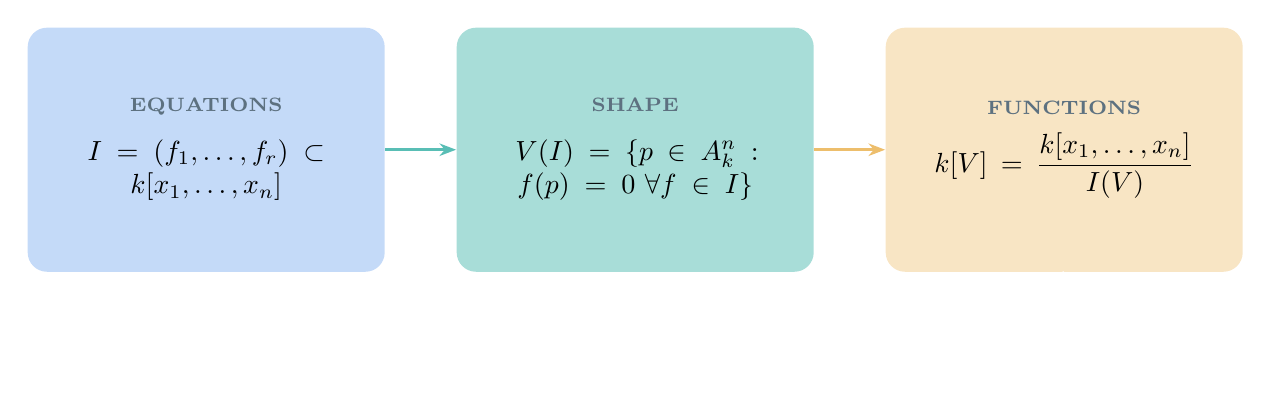
\begin{tikzpicture}[node distance=9mm]
  \node[rounded corners=7pt,fill=blue!28,text width=43mm,minimum height=31mm,align=center] (eq)
    {\tinycap{Equations}\vspace{3mm}\\[-1mm]
     $\displaystyle I=(f_1,\ldots,f_r)\subset \kk[x_1,\ldots,x_n]$};
  \node[rounded corners=7pt,fill=teal!34,text width=43mm,minimum height=31mm,align=center,right=of eq] (shape)
    {\tinycap{Shape}\vspace{3mm}\\[-1mm]
     $\displaystyle V(I)=\{p\in\A^n_{\kk}:f(p)=0\ \forall f\in I\}$};
  \node[rounded corners=7pt,fill=gold!30,text width=43mm,minimum height=31mm,align=center,right=of shape] (ring)
    {\tinycap{Functions}\vspace{3mm}\\[-1mm]
     $\displaystyle \kk[V]=\frac{\kk[x_1,\ldots,x_n]}{I(V)}$};
  \draw[-{Stealth[length=6pt]},line width=1.2pt,draw=teal!65!white] (eq)--(shape);
  \draw[-{Stealth[length=6pt]},line width=1.2pt,draw=gold!75!white] (shape)--(ring);
  \draw[-{Stealth[length=6pt]},line width=1pt,draw=white!55,bend left=35] (ring.south) to node[below,text=white!70,font=\scriptsize] {$\operatorname{Spec}$ reads algebra back as geometry} (shape.south);
\end{tikzpicture}
\end{center}

\vfill
{\fontsize{14}{16}\selectfont\bfseries The central equivalence}\par\vspace{3mm}
{\fontsize{10}{14}\selectfont\color{white!82}
A variety is a \textbf{zero set cut out by polynomials}. Its coordinate ring records the \textbf{polynomial functions that survive on that zero set}. Algebraic geometry gains its force by moving through this dictionary in both directions.\par}
\vspace{10mm}
{\fontsize{7}{8}\selectfont\color{white!58}
Prerequisites: polynomials, coordinates, and a little linear algebra\hfill Benjamin Michael Haire / 2026}
\newpage
\nopagecolor
\color{ink}

% PAGE 2
\renewcommand{\footertext}{ZERO SETS / AFFINE SPACE / THE BASE FIELD}
\pagehead{01}{ZERO SETS}{Equations become spaces}
\lead{Start with affine space $\A^n_{\kk}=\kk^n$. A polynomial does more than compute a number: its simultaneous zeros carve out a geometric object.}

\begin{mathbox}
\begin{align*}
V(f_1,\ldots,f_r)
  &=\bigl\{p=(a_1,\ldots,a_n)\in\A^n_{\kk}:f_i(p)=0\text{ for }1\le i\le r\bigr\},\\
I(X)
  &=\bigl\{f\in\kk[x_1,\ldots,x_n]:f(p)=0\text{ for every }p\in X\bigr\}.
\end{align*}
\end{mathbox}

\vspace{4pt}
\begin{minipage}[t]{.316\textwidth}
\begin{quietbox}
\textbf{Line}\hfill $V(y-x)$\par\vspace{2pt}
\begin{center}
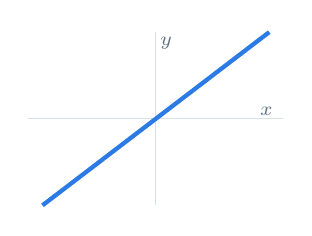
\begin{tikzpicture}[x=.72cm,y=.55cm]
  \draw[axis] (-2.25,0)--(2.25,0); \draw[axis] (0,-2)--(0,2);
  \draw[curveblue] (-2,-2)--(2,2);
  \node[font=\scriptsize,text=muted] at (1.95,.18) {$x$};
  \node[font=\scriptsize,text=muted] at (.18,1.75) {$y$};
\end{tikzpicture}
\end{center}
$t\mapsto(t,t)$ gives one free parameter, so the line has dimension $1$.
\end{quietbox}
\end{minipage}\hfill
\begin{minipage}[t]{.316\textwidth}
\begin{quietbox}
\textbf{Parabola}\hfill $V(y-x^2)$\par\vspace{2pt}
\begin{center}
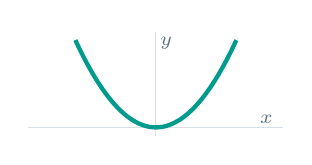
\begin{tikzpicture}[x=.72cm,y=.55cm]
  \draw[axis] (-2.25,0)--(2.25,0); \draw[axis] (0,-.2)--(0,2.2);
  \draw[curveteal,domain=-1.42:1.42,samples=70] plot (\x,{\x*\x});
  \node[font=\scriptsize,text=muted] at (1.95,.18) {$x$};
  \node[font=\scriptsize,text=muted] at (.18,1.95) {$y$};
\end{tikzpicture}
\end{center}
$t\mapsto(t,t^2)$ shows that a nonlinear picture may still have one parameter.
\end{quietbox}
\end{minipage}\hfill
\begin{minipage}[t]{.316\textwidth}
\begin{quietbox}
\textbf{Circle}\hfill $V(x^2+y^2-1)$\par\vspace{2pt}
\begin{center}
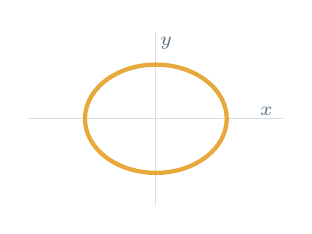
\begin{tikzpicture}[x=.72cm,y=.55cm]
  \draw[axis] (-2.25,0)--(2.25,0); \draw[axis] (0,-2)--(0,2);
  \draw[curvegold] (0,0) circle [x radius=1.25,y radius=1.25];
  \node[font=\scriptsize,text=muted] at (1.95,.18) {$x$};
  \node[font=\scriptsize,text=muted] at (.18,1.75) {$y$};
\end{tikzpicture}
\end{center}
One equation in two coordinates usually leaves one degree of freedom.
\end{quietbox}
\end{minipage}

\vspace{5pt}
\begin{goldbox}
\eyebrow{The field changes the geometry}\par\vspace{3pt}
\[
V_{\mathbb R}(x^2+y^2+1)=\varnothing,
\qquad
V_{\mathbb C}(x^2+y^2+1)\neq\varnothing.
\]
We draw real loci for intuition. The clean ideal-zero-set correspondence is strongest over an algebraically closed field, usually $\kk=\mathbb C$.
\end{goldbox}

\vspace{4pt}
\textbf{First habit.} Given equations, name the ambient space, the base field, and the common zero set before trying to picture it.
\newpage

% PAGE 3
\renewcommand{\footertext}{IDEALS / INTERSECTION AND UNION / RADICALS}
\pagehead{02}{MORE THAN ONE EQUATION}{Systems and ideals}
\lead{A system means simultaneous vanishing. Geometrically, this is intersection. Algebraically, every polynomial consequence is packaged into an ideal.}

\begin{minipage}[t]{.46\textwidth}
\begin{quietbox}
\textbf{Solve a circle-line intersection}\par\vspace{3pt}
\begin{center}
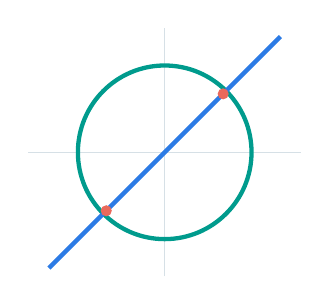
\begin{tikzpicture}[x=1.05cm,y=1.05cm]
  \draw[axis] (-1.65,0)--(1.65,0); \draw[axis] (0,-1.5)--(0,1.5);
  \draw[curveteal] (0,0) circle (1.05);
  \draw[curveblue] (-1.4,-1.4)--(1.4,1.4);
  \fill[coral] ({1/sqrt(2)},{1/sqrt(2)}) circle (2pt);
  \fill[coral] ({-1/sqrt(2)},{-1/sqrt(2)}) circle (2pt);
\end{tikzpicture}
\end{center}
\begin{align*}
x^2+y^2-1&=0, & y-x&=0,\\
2x^2&=1, & y&=x,\\
(x,y)&=\left(\pm\frac1{\sqrt2},\pm\frac1{\sqrt2}\right).
\end{align*}
The signs are paired: the intersection has exactly two points.
\end{quietbox}
\end{minipage}\hfill
\begin{minipage}[t]{.50\textwidth}
\begin{mathbox}
\[
I=(f_1,\ldots,f_r)
=\left\{\sum_{i=1}^{r}h_i f_i:h_i\in\kk[x_1,\ldots,x_n]\right\}.
\]
Every element of $I$ vanishes wherever $f_1,\ldots,f_r$ vanish.
\end{mathbox}
\vspace{5pt}
\begin{align*}
V(I+J)&=V(I)\cap V(J),\\
V(IJ)&=V(I)\cup V(J),\\
I(X\cup Y)&=I(X)\cap I(Y).
\end{align*}
More equations produce fewer points. More geometric points leave fewer polynomials vanishing everywhere.
\end{minipage}

\vspace{6pt}
\begin{coralbox}
\eyebrow{The zero set forgets powers}\par\vspace{2pt}
\[
V(x)=V(x^2),\qquad (x)\neq(x^2).
\]
The radical removes multiplicity that the underlying point set cannot see:
\[
\sqrt I=\{g:g^m\in I\text{ for some }m\ge1\}.
\]
Over an algebraically closed field, Hilbert's Nullstellensatz closes the dictionary:
\[
\boxed{\ I(V(I))=\sqrt I\ }.
\]
\end{coralbox}

\vspace{5pt}
\begin{tealbox}
\textbf{Two quick decompositions}
\begin{align*}
V(xy)&=V(x)\cup V(y),\\
V\bigl((y-x)(y+x)\bigr)&=V(y-x)\cup V(y+x).
\end{align*}
A reducible polynomial often reveals a reducible geometric set.
\end{tealbox}
\newpage

% PAGE 4
\renewcommand{\footertext}{TANGENT SPACES / GRADIENTS / THE JACOBIAN}
\pagehead{03}{ZOOM IN}{Local geometry and singularities}
\lead{At a smooth point, the first-order terms capture the local shape. At a singular point, the linear approximation loses rank and higher-order terms become visible.}

\begin{mathbox}
For $F=(f_1,\ldots,f_r):\A^n\to\A^r$, define
\[
J_F(p)=\left(\frac{\partial f_i}{\partial x_j}(p)\right)_{i,j},
\qquad
T_pV=\ker J_F(p),
\qquad
\dim T_pV=n-\rank J_F(p).
\]
For a hypersurface $V(f)$, smoothness at $p$ is the condition $\nabla f(p)\neq0$.
\end{mathbox}

\vspace{5pt}
\begin{minipage}[t]{.485\textwidth}
\begin{quietbox}
\textbf{Smooth point on a circle}\hfill $f=x^2+y^2-1$\par
\begin{center}
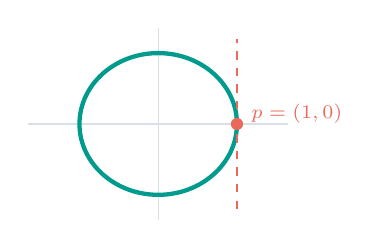
\begin{tikzpicture}[x=1.0cm,y=.9cm]
  \draw[axis] (-1.65,0)--(1.65,0); \draw[axis] (0,-1.35)--(0,1.35);
  \draw[curveteal] (0,0) circle (1);
  \draw[tangent] (1,-1.2)--(1,1.2);
  \fill[coral] (1,0) circle (2.2pt);
  \node[font=\scriptsize,text=coral,anchor=west] at (1.06,.15) {$p=(1,0)$};
\end{tikzpicture}
\end{center}
\begin{align*}
\nabla f&=(2x,2y), & \nabla f(1,0)&=(2,0),\\
T_pV&:\ 2(x-1)=0, & &x=1.
\end{align*}
The gradient is normal to the tangent line.
\end{quietbox}
\end{minipage}\hfill
\begin{minipage}[t]{.485\textwidth}
\begin{quietbox}
\textbf{Singular cusp}\hfill $f=y^2-x^3$\par
\begin{center}
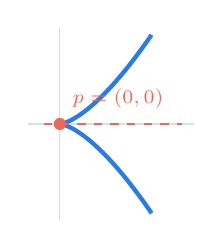
\begin{tikzpicture}[x=1.0cm,y=.9cm]
  \draw[axis] (-.4,0)--(1.7,0); \draw[axis] (0,-1.35)--(0,1.35);
  \draw[curveblue,domain=-1.08:1.08,samples=90] plot ({\x*\x},{\x*\x*\x});
  \draw[tangent] (-.2,0)--(1.55,0);
  \fill[coral] (0,0) circle (2.2pt);
  \node[font=\scriptsize,text=coral,anchor=south west] at (.04,.08) {$p=(0,0)$};
\end{tikzpicture}
\end{center}
\begin{align*}
\nabla f&=(-3x^2,2y), & \nabla f(0,0)&=(0,0),\\
T_pV&=\A^2, & \dim T_pV&=2>\dim V.
\end{align*}
The lowest-degree term is $y^2$, giving the doubled tangent direction $y=0$.
\end{quietbox}
\end{minipage}

\vspace{6pt}
\begin{goldbox}
\eyebrow{Expected rank is the practical test}\par\vspace{2pt}
If $r$ independent equations cut out a local piece of codimension $r$, then a smooth point satisfies
\[
\rank J_F(p)=r,
\qquad
\dim T_pV=n-r.
\]
A rank drop signals a singularity, a component crossing, or a degeneration that deserves closer inspection.
\end{goldbox}
\newpage

% PAGE 5
\renewcommand{\footertext}{QUOTIENT RINGS / FUNCTIONS / THE ALGEBRA-GEOMETRY DICTIONARY}
\pagehead{04}{TURN GEOMETRY INTO ALGEBRA}{The coordinate ring}
\lead{Two polynomials define the same function on a variety when their difference vanishes there. Quotienting by those relations produces the ring of polynomial functions on the shape.}

\begin{mathbox}
\begin{align*}
\kk[V]&=\frac{\kk[x_1,\ldots,x_n]}{I(V)},\\
f|_V=g|_V&\Longleftrightarrow f-g\in I(V).
\end{align*}
The class $[f]\in\kk[V]$ is the polynomial function induced by $f$ on $V$.
\end{mathbox}

\vspace{5pt}
\begin{center}
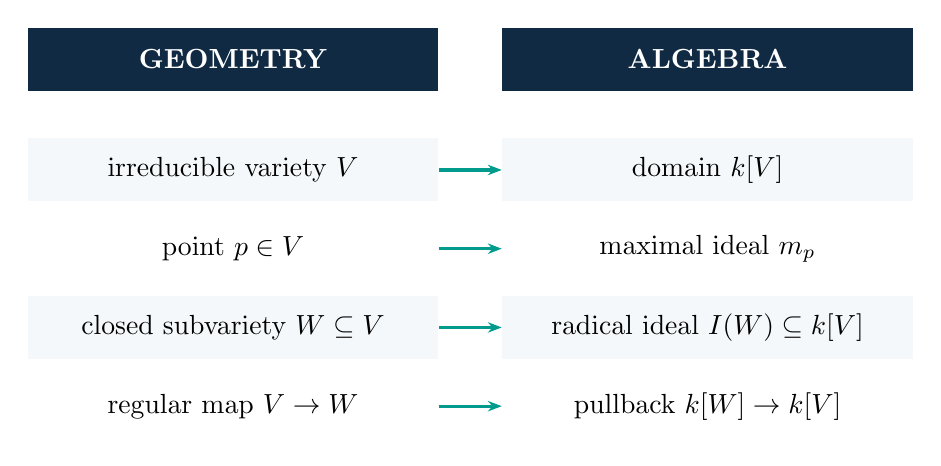
\begin{tikzpicture}[node distance=3.5mm]
\node[fill=navy,text=white,minimum width=.43\textwidth,minimum height=8mm,font=\bfseries] (g0) {GEOMETRY};
\node[fill=navy,text=white,minimum width=.43\textwidth,minimum height=8mm,font=\bfseries,right=8mm of g0] (a0) {ALGEBRA};
\foreach \i/\lefttext/\righttext in {
1/{irreducible variety $V$}/{domain $\kk[V]$},
2/{point $p\in V$}/{maximal ideal $\mathfrak m_p$},
3/{closed subvariety $W\subseteq V$}/{radical ideal $I(W)\subseteq\kk[V]$},
4/{regular map $V\to W$}/{pullback $\kk[W]\to\kk[V]$}}
{
  \node[below=\i*10mm of g0,anchor=center,minimum width=.43\textwidth,minimum height=8mm,fill=\ifodd\i pale\else white\fi] (g\i) {\lefttext};
  \node[below=\i*10mm of a0,anchor=center,minimum width=.43\textwidth,minimum height=8mm,fill=\ifodd\i pale\else white\fi] (a\i) {\righttext};
  \draw[flow] (g\i.east)--(a\i.west);
}
\end{tikzpicture}
\end{center}

\vspace{3pt}
\begin{tealbox}
\begin{minipage}[t]{.34\textwidth}
\eyebrow{Example: the hyperbola}\par\vspace{3pt}
\begin{center}
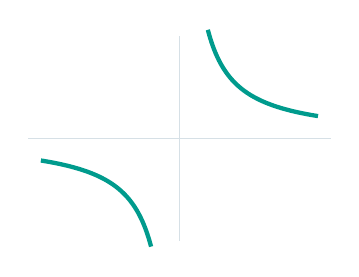
\begin{tikzpicture}[x=.8cm,y=.62cm]
  \draw[axis] (-2.4,0)--(2.4,0); \draw[axis] (0,-2.1)--(0,2.1);
  \draw[curveteal,domain=.45:2.2,samples=60] plot (\x,{1/\x});
  \draw[curveteal,domain=-2.2:-.45,samples=60] plot (\x,{1/\x});
\end{tikzpicture}
\end{center}
\end{minipage}\hfill
\begin{minipage}[t]{.61\textwidth}
Let $H=V(xy-1)$. In its coordinate ring, $[x][y]=1$, so $[x]$ is invertible:
\begin{align*}
\kk[H]
  &=\frac{\kk[x,y]}{(xy-1)}
    \cong \kk[x,x^{-1}],\\
[x]&\longmapsto x,
&[y]&\longmapsto x^{-1}.
\end{align*}
The equation has become an algebraic rule: $x$ never vanishes on $H$.
\end{minipage}
\end{tealbox}

\vspace{4pt}
{\small For irreducible $V$, the coordinate ring is a domain and
$\displaystyle \dim V=\trdeg_{\kk}\Frac(\kk[V])$, the number of algebraically independent rational parameters.}
\newpage

% PAGE 6
\renewcommand{\footertext}{REGULAR MAPS / PULLBACK / PARAMETRIZATION / NORMALIZATION}
\pagehead{05}{POLYNOMIAL MOTION}{Maps between varieties}
\lead{A regular map moves points forward by polynomial formulas. Functions move backward by composition. This contravariance is the organizing rhythm of the subject.}

\begin{mathbox}
\begin{align*}
\varphi:V&\longrightarrow W,
&p&\longmapsto\bigl(\varphi_1(p),\ldots,\varphi_m(p)\bigr),\\
\varphi^*:\kk[W]&\longrightarrow\kk[V],
&h&\longmapsto h\circ\varphi,\\
(\psi\circ\varphi)^*&=\varphi^*\circ\psi^*.
\end{align*}
\end{mathbox}

\vspace{5pt}
\begin{quietbox}
\begin{minipage}[t]{.42\textwidth}
\eyebrow{The parabola is the affine line}\par\vspace{4pt}
\[
\varphi:\A^1\to V(y-x^2),\qquad t\mapsto(t,t^2).
\]
The pullback is an isomorphism:
\[
\varphi^*:\frac{\kk[x,y]}{(y-x^2)}\xrightarrow{\sim}\kk[t],
\qquad [x]\mapsto t,\ [y]\mapsto t^2.
\]
Its inverse sends $t\mapsto[x]$.
\end{minipage}\hfill
\begin{minipage}[t]{.52\textwidth}
\begin{center}
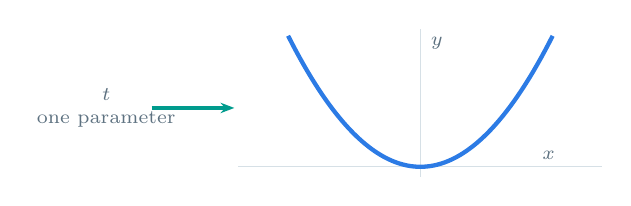
\begin{tikzpicture}[x=1.05cm,y=.65cm]
  \draw[axis] (-2.2,0)--(2.2,0); \draw[axis] (0,-.2)--(0,2.7);
  \draw[curveblue,domain=-1.6:1.6,samples=70] plot (\x,{\x*\x});
  \draw[flow] (-3.25,1.15)--(-2.25,1.15);
  \node[font=\scriptsize,align=center,text=muted] at (-3.8,1.15) {$t$\\one parameter};
  \node[font=\scriptsize,text=muted] at (1.55,.22) {$x$};
  \node[font=\scriptsize,text=muted] at (.2,2.42) {$y$};
\end{tikzpicture}
\end{center}
\end{minipage}
\end{quietbox}

\vspace{6pt}
\begin{coralbox}
\begin{minipage}[t]{.35\textwidth}
\eyebrow{The cusp trap}\par\vspace{4pt}
\begin{center}
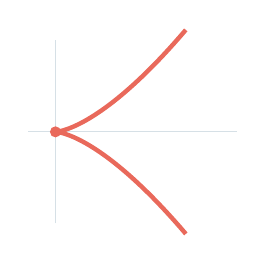
\begin{tikzpicture}[x=1.15cm,y=.75cm]
  \draw[axis] (-.3,0)--(2.0,0); \draw[axis] (0,-1.55)--(0,1.55);
  \draw[draw=coral,line width=1.6pt,domain=-1.2:1.2,samples=90] plot ({\x*\x},{\x*\x*\x});
  \fill[coral] (0,0) circle (2pt);
\end{tikzpicture}
\end{center}
\end{minipage}\hfill
\begin{minipage}[t]{.60\textwidth}
The map $\nu(t)=(t^2,t^3)$ is bijective onto $C=V(y^2-x^3)$, but
\[
\nu^*:\frac{\kk[x,y]}{(y^2-x^3)}\hookrightarrow\kk[t],
\qquad [x]\mapsto t^2,\ [y]\mapsto t^3
\]
has image $\kk[t^2,t^3]\neq\kk[t]$. The missing function $t$ would equal $y/x$ away from the origin, but $y/x$ is not regular at the cusp. Thus $\nu$ is the \textbf{normalization}, not an isomorphism.
\end{minipage}
\end{coralbox}
\newpage

% PAGE 7
\renewcommand{\footertext}{PROJECTIVE SPACE / HOMOGENIZATION / POINTS AT INFINITY}
\pagehead{06}{ADD POINTS AT INFINITY}{Why projective space appears}
\lead{Affine space hides limiting directions. Projective space adds them and makes polynomial geometry more complete.}

\begin{mathbox}
\[
\Pj^n(\kk)=\frac{\kk^{n+1}\setminus\{0\}}{\kk^\times},
\qquad
[X_0:\cdots:X_n]=[\lambda X_0:\cdots:\lambda X_n]\quad(\lambda\neq0).
\]
Projective varieties are cut out by homogeneous polynomials, whose monomials all have the same total degree.
\end{mathbox}

\vspace{5pt}
\begin{minipage}[t]{.47\textwidth}
\begin{quietbox}
\eyebrow{Homogenize the parabola}\par\vspace{4pt}
In the affine chart $Z\neq0$, write $x=X/Z$ and $y=Y/Z$:
\begin{align*}
y-x^2&=0,\\
\frac{Y}{Z}-\frac{X^2}{Z^2}&=0,\\
YZ-X^2&=0.
\end{align*}
At infinity, $Z=0$, so $X=0$. The projective closure gains one point:
\[
\overline{V(y-x^2)}\cap\{Z=0\}=\{[0:1:0]\}.
\]
\end{quietbox}
\end{minipage}\hfill
\begin{minipage}[t]{.49\textwidth}
\begin{center}
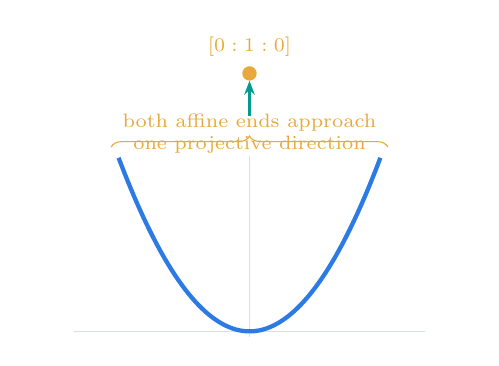
\begin{tikzpicture}[x=.95cm,y=.72cm]
  \draw[axis] (-2.35,0)--(2.35,0); \draw[axis] (0,-.1)--(0,3.1);
  \draw[curveblue,domain=-1.75:1.75,samples=70] plot (\x,{\x*\x});
  \draw[decorate,decoration={brace,amplitude=4pt},draw=gold] (-1.85,3.25)--(1.85,3.25);
  \node[font=\scriptsize,text=gold,text width=54mm,align=center] at (0,3.48) {both affine ends approach one projective direction};
  \draw[flow] (0,3.80)--(0,4.42);
  \fill[gold] (0,4.55) circle (2.6pt);
  \node[font=\scriptsize\bfseries,text=gold,anchor=south] at (0,4.68) {$[0:1:0]$};
\end{tikzpicture}
\end{center}
\begin{goldbox}
\textbf{A second example}
\begin{align*}
xy-1&\rightsquigarrow XY-Z^2,\\
Z=0&\Longrightarrow XY=0.
\end{align*}
The hyperbola gains two points at infinity: $[1:0:0]$ and $[0:1:0]$.
\end{goldbox}
\end{minipage}

\vspace{6pt}
\begin{tealbox}
\eyebrow{Why the completion matters}\par\vspace{3pt}
\begin{multicols}{3}
\textbf{Intersections}\par
Curves that appear parallel in an affine chart can meet at infinity.

\columnbreak
\textbf{Completeness}\par
Projective varieties behave like compact spaces in algebraic geometry.

\columnbreak
\textbf{Degree}\par
Homogeneous equations make intersection counts and scaling symmetries visible.
\end{multicols}
\end{tealbox}

\vspace{3pt}
{\small For example, Bezout's theorem predicts that two projective plane curves of degrees $d$ and $e$, with no common component, meet in $de$ points counted with multiplicity over an algebraically closed field.}
\newpage

% PAGE 8
\renewcommand{\footertext}{DIMENSION / IRREDUCIBILITY / YOUR NEXT PROBLEM}
\pagehead{07}{A REUSABLE MENTAL MODEL}{The whole picture}
\lead{Algebraic geometry is a method: cut out a space, inspect its local geometry, encode its functions, study its maps, and complete it when infinity matters.}

\begin{center}
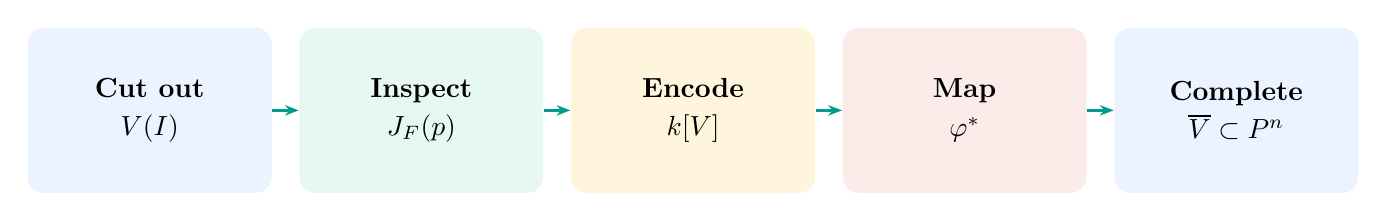
\begin{tikzpicture}[node distance=3mm]
\foreach \x/\title/\math/\fillc in {
0/Cut out/$V(I)$/paleblue,
1/Inspect/$J_F(p)$/paleteal,
2/Encode/$\kk[V]$/palegold,
3/Map/$\varphi^*$/palecoral,
4/Complete/$\overline V\subset\Pj^n$/paleblue}
{
\node[rounded corners=6pt,fill=\fillc,minimum width=31mm,minimum height=21mm,align=center] (n\x) at (\x*3.45,0)
{\textbf{\title}\\[2pt]\math};
}
\foreach \x in {0,1,2,3}{\draw[flow] (n\x.east)--(n\the\numexpr\x+1\relax.west);}
\end{tikzpicture}
\end{center}

\vspace{5pt}
\begin{quietbox}
\eyebrow{Three words to keep}\par\vspace{3pt}
\begin{align*}
\dim V&=\text{number of independent local parameters},\\
V\text{ irreducible}
&\Longleftrightarrow V\neq X\cup Y\text{ for proper closed }X,Y
\Longleftrightarrow \kk[V]\text{ is a domain},\\
\text{variety}
&=\text{an irreducible algebraic set in the convention used here.}
\end{align*}
Some texts allow reducible varieties and reserve \emph{integral variety} for the irreducible, reduced case.
\end{quietbox}

\vspace{6pt}
{\fontsize{13}{15}\selectfont\bfseries\color{navy}Four quick checks}\par\vspace{5pt}
\begin{minipage}[t]{.485\textwidth}
\textbf{1. Decompose $V(xy)\subset\A^2$.}\par
\begin{tealbox}
\[
V(xy)=V(x)\cup V(y),
\]
the two coordinate axes.
\end{tealbox}
\vspace{5pt}
\textbf{3. Homogenize $xy=1$.}\par
\begin{goldbox}
\[
XY=Z^2,\qquad Z=0\Longrightarrow [1:0:0],[0:1:0].
\]
\end{goldbox}
\end{minipage}\hfill
\begin{minipage}[t]{.485\textwidth}
\textbf{2. Find the singular locus of $y^2=x^3$.}\par
\begin{coralbox}
\[
(-3x^2,2y)=(0,0)\Longrightarrow (x,y)=(0,0).
\]
\end{coralbox}
\vspace{5pt}
\textbf{4. Invert $t\mapsto(t,t^2)$.}\par
\begin{mathbox}
\[
(x,y)\longmapsto x,
\]
a regular inverse on $V(y-x^2)$.
\end{mathbox}
\end{minipage}

\vspace{6pt}
\begin{mathbox}
\centering
\textbf{The compact dictionary}\qquad
$I\mapsto V(I)$,
$X\mapsto I(X)$,
$V\mapsto\kk[V]$,
$\varphi\mapsto\varphi^*$,
$f\mapsto f^{\mathrm h}$.
\end{mathbox}

\vfill
\eyebrow{Next}\quad
Cox, Little, and O'Shea for computation; Harris or Gathmann for the geometric theory.

\end{document}
